%Path planning for informational effect: pose uncertainty}
%---------------------------------------------------------------------------------------------------------------------
% 	ABSTRACT
%---------------------------------------------------------------------------------------------------------------------
%---------------------------------------------------------------------------------------------------------------------

Chapter~\ref{ch04} has shown that decision-theoretical frameworks can be extended to domains in which the agent has no perfect sensing abilities. This is a typical situation in robotics, where a robot perceives the world through noisy sensors. To perform tasks in such environments, a robot has to be capable of gathering information to recover its knowledge of the world, if necessary.

This chapter shows how to reason about information effects to refine the localisation of the object to be grasped when the object is not in the expected pose.
The main novel outcome is thus to enable tactile information gain planning for dexterous, high degree of freedom (DoF) manipulators. This is achieved by using a combination of  information gain planning, hierarchical probabilistic roadmap planning, and belief updating from tactile sensors for objects with non-Gaussian pose uncertainty in 6 dimensions. 

In this chapter it will be assumed that a single object with a known shape model is available as well as a desired robot grasp configuration with respect to the object. This means that only the pose of the object is uncertain. In addition, the algorithm will treat subsequent reach-to-grasp problems as independent. this means that the robot manipulator will be withdrawn to a safe position before re-planning the next reach-to-grasp trajectory. In the next chapter, we will discuss how to relax some of these assumptions. 

In this chapter, the method is demonstrated in trials with simulated robots. Sequential re-planning is shown to achieve a greater success rate than single grasp attempts, and trajectories that maximise information gain require fewer re-planning iterations than conventional planning methods before a grasp is achieved.

%---------------------------------------------------------------------------------------------------------------------
% 	ROADMAP
%---------------------------------------------------------------------------------------------------------------------
%---------------------------------------------------------------------------------------------------------------------
\section{Organisation}

This chapter proceeds as follows. Section~\ref{sec:ch06:introduction} presents the problem of planning a reach-to-grasp trajectory for dexterous robot manipulators under uncertainty on the pose of the object to be grasped. A main contribution of this thesis is that of building solutions that simultaneously attempt to perform a task (here dexterous grasping) as well as gather information (i.e. locate the object to be grasped), if necessary.

Section~\ref{sec:ch06:problem_domain} presents an alternative formulation for the problem of planning grasping under uncertainty. Instead of formalising it as an ISMDP problem, I pose the problem as an optimisation problem. 
%This section will i) describe how to iteratively update localisation knowledge using tactile observations from a previous grasp attempt, ii) show how successive grasp trajectories can be planned with respect to these iteratively refined object poses, and iii) show how each reach-to-grasp trajectory can be deliberately planned to maximise new tactile information gain, while also reaching towards the expected grasp location derived from previous information. 

Section~\ref{sec:ch06:solution_domain} discusses the implementation details of my proposed approach.

Section~\ref{sec:ch06:results} presents experimental test results in which a dexterous grasping trajectory has to be planned under non-Gaussian object-pose uncertainty in 6D. Three strategies are presented. 
%The results shows that sequential re-planning algorithms are capable to achieve a grasp with higher successful rate, and that maximising information gain along the trajectories yields to fewer re-planning iterations.

Section~\ref{sec:ch06:summary} summarises the contributions of this chapters. 

%---------------------------------------------------------------------------------------------------------------------
% 	INTRO
%---------------------------------------------------------------------------------------------------------------------
%---------------------------------------------------------------------------------------------------------------------

\section{Introduction}\label{sec:ch06:introduction}

As described in Sec.~\ref{sec:ch01_approach_grasping}, robot grasping is typically affected by uncertainty associated with the location of the object to be grasped.  
This is a challenging problem because requires us to find collision-free trajectories in a high-dimensional space (the robot's joint space, Sec.~\ref{sec:ch03:configspace}) as well as to reason about how to act more robustly in the face of such an uncertainty. Section~\ref{sec:ch02:grasp_planning} has reviewed previous work on planning dexterous grasping under object pose uncertainty. Typically these efforts are based on the separation of information gathering trajectories from grasping trajectories. 

The main contributions of this work are:
\begin{itemize}
\item Planning information gain trajectories whilst simultaneously attempting to grasp the target object.
\item Using a hierarchical sample-based path planner, here a Probabilistic Roadmap (PRM) planner, which encodes expected information gain (in a low-dimensional belief space) in its trajectory segments.
\item Refining the expected object pose by using an observation model for contact sensing by a multi-finger hand that palpates a 3D object to be grasped.
\item Showing that this approach enables planning for robot manipulators with 21 DoF and non-Gaussian object pose uncertainty in 6 dimensions.
\end{itemize}
%extending a sample-based path planner, here a PRM planner, to efficiently plan dexterous reach-to-grasp trajectories for high DoF manipulators ii) embedding an informational measure in the trajectory segments considered by our PRM-based planner, and iii) creating an observation model for contact sensing by a multi-finger hand that palpates the object to be grasped. 

Several assumptions are made. First, the object is of known shape, in the sense that a high density point cloud model or mesh model is available. Second, a pre-computed grasp (i.e. a set of finger contacts) and its pre-grasp configuration are known a priori for this object. Third, the algorithm assumes the availability of an unreliable estimate of the object's pose. In addition, each re-planning iteration is treated as independent and thus the robot's manipulator was withdrawn to a safe position after a failed attempt to grasp, and the (tactile) sensing abilities of the robot are assumed to be perfect (no false detections).

In this scenario (shown in Fig.~\ref{fig:spam.example}), a depth image is obtained from an Asus Xtion Pro depth camera. This gives an incomplete point cloud of the object surface, I refer to this new point cloud as a \emph{query point cloud} or simply \emph{query} to distinguish it from the point cloud used as the \emph{model}. Using a model fitting procedure similar to the sampling from surflet pairs method presented in~\citep{bib:uli_cviu_2011}, a probability density (or belief state) over the object pose is estimated, represented as a particle set. Given this distribution, a reach-to-grasp trajectory is planned. This trajectory has as its goal configuration the pre-computed grasp under the assumption that the object is at a pose corresponding to the mean position of the particle set. The path to this goal configuration is found using a stochastic motion planner. This planner works with a cost function that allows deviations from the shortest path that maximise the chance of gathering tactile observations that will reduce pose uncertainty in the object location. If unexpected observations occurred during the execution of the planned trajectory, then such observations (both tactile contact and no-contact signals) collected at poses along the reach-to-grasp trajectory are used to perform a particle filter update. Re-planning then occurs with the new pose distribution, and a new reach-to-grasp trajectory can be constructed. This process is then iterated until a successful grasp is achieved.
	
\begin{figure}[!t]
\centerline{
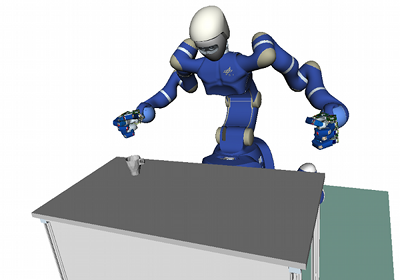
\includegraphics[height=5.0cm,width=.48\columnwidth]{../media/iros/2013/img/from_rss/justin_grasp_example}
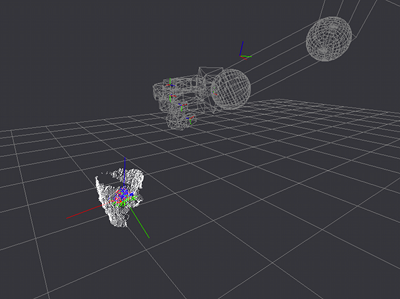
\includegraphics[height=5.0cm,width=.48\columnwidth]{../media/iros/2013/img/from_rss/partial_point_cloud}
}
\caption[Grasp example:]{Justin and a known mug to grasp in OpenRave simulator (left). Partial point cloud of the mug used for localisation (right).}
\label{fig:spam.example}
\end{figure}

In Sec.~\ref{sec:ch04:remarks_pomdp}, we discussed the benefits of planning in belief spaces as well as its limitations in real world applications. 
Thus, this work is related to the approach of the approach of Platt et al.~\citep{bib:platt_csail_2011}, ~\citep{bib:platt_icra_2012} (discussed in more details in Sec.~\ref{sec:ch02:grasp_planning}). That work plans a sequence of actions that will generate observations that distinguish a hypothesised state from competing hypotheses while also reaching a goal position. The informational value of a trajectory is the difference in the expected observations between the hypothesised position and each alternative. This approach allows us to track high-dimensional belief states using an accurate filter defined by the user, but reduces the complexity of planning in belief spaces by approximating the informational value of actions from a low-dimensional subspace of the belief state. Platt et al. applied this to planning for a two degree of freedom manipulator using a laser range finder for observations, and employed an optimisation framework for planning. The algorithm is proved to localise the true state of the system in 1 dimension and to reach a goal region with high probability. In contrast to~\citep{bib:platt_csail_2011}, my approach encodes information gathering actions to localise an object to be grasped in 6 dimensions while simultaneously attempting to achieve the task of grasping.  Similarly to~\citep{bib:platt_csail_2011},~\citep{bib:platt_icra_2012}, this method is guaranteed to converge to the true state of the system in which a reach-to-grasp trajectory succeeds with high probability, under the assumption that the system is not perturbed by previous grasping attempts (e.g. the robot contacts the target object without changing its configuration). Here we also discuss how this approach can be extended to planning the motion of a manipulator performing multi-finger grasping. 

\begin{figure}[!t]
\centerline{
\includegraphics[height=5.0cm,width=.48\columnwidth]{../media/iros/2013/img/justin_small.png}
\includegraphics[height=5.0cm,width=.48\columnwidth]{../media/iros/2013/img/justin_small2.png}
}
\caption[Real scenario]{Rollin Justin at DLR. Justin in a starting configuration, the mug to be grasped (glued on the desk) and the depth camera (left). Justin executing a successful reach-to-grasp trajectory which leads to grasp the mug (right). Since the mug is glued on the desk, Justin cannot lift it up to prove the real stability of the grasp.}
\label{fig:justin}
\end{figure}

This approach has been tested in simulation, as described in Sec.~\ref{sec:ch01:grasping_scenario_gert}. 
%Since physics-based simulators are hard to calibrate, I use i) a Nvidia Physx-based simulator~\citep{bib:kopicki_2010}, and ii) OpenRave-based,~\citep{bib:rosen_2008}, Justin Simulator developed at DLR for control and visualisation of the entire robot~\citep{bib:fuchs_2009}. Both simulators interface with a Bullet-based simulator developed at DLR, which is accurately calibrated to simulate hand-object physical interactions. I use the Bullet simulator to simulate contacts and compute grasp quality measure. For proof of concept, we also tested this approach on the Rollin Justin robot. However, in order to guarantee no movement after a contact, the object to be grasped needed to be glued on the desk. Therefore even though this approach converged to a force closure grasp, Rollin Justin could not lift up the object to prove the real stability of the grasp. %We argue that with finer tactile sensors on Rollin Justin's end-effector we would be able to sense an object and converge to a robust grasp without need to glue it on the desk.
The following section introduces the formulation of the problem of planning grasping under uncertainty used in this thesis.

%---------------------------------------------------------------------------------------------------------------------
% 	PROBLEM DOMAIN
%---------------------------------------------------------------------------------------------------------------------
%---------------------------------------------------------------------------------------------------------------------
\section{Planning trajectory}\label{sec:ch06:problem_domain}

This chapter presents a formulation to the problem of planning dexterous grasping trajectories under object pose uncertainty using information gain re-planning. First I show
how tactile information, acquired during a failed attempt to grasp an object can be used to refine the estimate of that object's pose, and then how this information can be used to re-plan new reach-to-grasp trajectories for successive grasp attempts. Finally I show how reach-to-grasp trajectories can be modified, so that they maximise the expected tactile information gain, while simultaneously delivering the hand to the grasp configuration that is most likely to succeed. 

%brief intro
%- we solve the problem of planning reach-and-grasp trajectories under non-Gaussian pose uncertainty, assuming we know the shape and the grasp
%- if we have a grasp in the object frame, the problem is to estimate where is the object in order to plan the action. with non-Gaussian uncertainty an open-loop planner which tries to grasp the object in the ML pose might fail
%- we assume the object is heavy enough not to be moved (static condition of the object)
%- we use only f/t/ sensors
%- the idea would be broadly applicable with everyday objects if using compliance hands with tactile sensors 



\subsection{Problem formulation}
%
%- mainly in real-world problem inferring the pose of an object produces a non-Gaussian pdf
%- introduction of (with some maths)
%-- transition function
%-- observation function
%-- objective function we want to minimise

This chapter is concerned with the problem of planning control actions to reach a goal state in the presence of incomplete or noisy observations. 
Let us consider a discrete-time system with continuous non-linear deterministic dynamics, 
$$
x_{t+1}=f(x_t,u_t) 
$$ 
where $x_{t}\in\mathbb{R}^n$ is a configuration state of the robot and $u_{t}\in\mathbb{R}^l$ is a action vector, both parametrised over time $t\in\{1,2,...\}$.
Let $p\in SE(3)$ describe the object pose, given an initial prior belief state $b_1$ and let us define a set of $k$ hypotheses as $\{p^i\}_{i=1}^k$, where $p^1=\arg\max b_1$ and $p^i\sim b_1,i\in[2,k]$. The idea is to search for a sequence of actions, $u_{1:T-1}=\{u_1,\dots,u_{T-1}\}$, that distinguish between observations that would occur if the object were in $p^1$ from any other $p^i$ pose, with $i\in[2,k]$.
At each time step, $t$, the system makes an observation, $y\in\mathbb{R}^m$, that is a non-linear stochastic function of states and hypotheses. 
%$$
%y_t=g(x_t,p^i)
%$$
%where $i\in[1,k]$. 
Without losing generality, we define $y_t$ to be a column vector of binary values. Each of these values represents whether or not a contact is observed between a given link of the robot and the hypothesis $p^i$.
However, binary values have been shown to be not very informative during the planning phase. Therefore let us define,
$$
h(x,p^i)=Pr(y=1|x,p^i)
$$
as a column vector of scores identifying the likelihood of observing a contact, $y=1$, as function of states and hypotheses.
More generally, let $F_t(x,u_{1:t-1})$ be the robot configuration at time $t$ if the system begins at state $x$ and takes action $u_{1:t-1}$. Therefore the expected sequence of observations over a trajectory, $u_{1:t-1}$, is:
$$
h_t(x,u_{1:t-1},p^i)=(h(F_2(x,u_1),p^i)^T,h(F_3(x,u_{1:2}),p^i)^T,\ldots,h(F_t(x,u_{1:t-1}),p^i)^T)^T
$$
a column vector which describes the likelihood of observing a contact at any time step of the trajectory $u_{1:t-1}$.
We then need to search for a sequence of actions which maximise the difference between observations that are expected to happen in the sampled states, $p^{2:k}$, when the system is actually in the most likely hypothesis, $p^1$. In other words, we want to find a sequence of action, $u_{1:T-1}$, that minimises
\begin{equation}\label{eq:cost}
\mathcal{J}(x,u_{1:T-1},p^{1:k})=\sum_{i=2}^kN(h(x,u_{1:T-1},p^i)|h(x,u_{1:T-1},p^1),\mathbb{Q})
\end{equation}
where $N(\cdot|\mu,\Sigma)$ denotes the Gaussian distribution with mean $\mu$ and covariance $\Sigma$ and $\mathbb{Q}$ is the block diagonal of measurement noise covariance matrices of appropriate size. Rather than optimising~(\ref{eq:cost}) we follow the suggested simplifications described in~\citep{bib:platt_csail_2011} by dropping the normalisation factor in the Gaussian and optimising the exponential factor only. Let us define for any $i\in[2,k]$
$$
\Phi(x,u_{1:T-1},p^i)=||h_t(x,u_{1:T-1},p^i)-h_t(x,u_{1:T-1},p^1)||_{\mathbb{Q}}^2,
$$
then the modified cost function is
\begin{equation}\label{eq:modifiedcost1}
\mathcal{J}(x,u_{1:T-1},p^{1:k})=\frac{1}{k}\sum_{i=2}^k{e^{-\Phi(x,u_{1:T-1},p^i)}}
\end{equation}
it is worth to notice that when there is a significant difference between the sequence of expected observations, $h_t(x,u_{1:T-1},p^i)$ and $h_t(x,u_{1:T-1},p^1)$, the function $\Phi(\cdot)$ is large and therefore $\mathcal{J}(\cdot)$ is small. On the other hand if the sequence of expected observations are very similar to each other, their distance measurement tends to 0 and $\mathcal{J}(\cdot)$ tends to 1.
Equation~(\ref{eq:modifiedcost1}) can be minimised using different planning techniques such as Randomly-exploring Random Trees (RRTs)~\citep{bib:lavalle_1998}, Probabilistic Roadmap (PRM)~\citep{bib:kavraki_1996}, Differential Dynamic Programming (DDP)~\citep{bib:jacobson_book_1970} or Sequential Dynamic Programming (SDP)~\citep{bib:betts_book_2001}. 
In Section~\ref{sec:ch06:heuristic}, we define a new set of heuristics that can be encoded in a PRM planner for generating more reliable trajectories that explicitly reason over the pose uncertainty, and demonstrate the method with experiments on a virtual testbed.

\subsection{Mean pose estimate}\label{sec:ch06:state_estimator}

As mentioned before, the sequential re-planning approach presented in this thesis assumes the availability of an unreliable estimate of the object's pose to construct a grasping trajectory.
In sec.~\ref{sec:ch02:state_estimate} we discussed the advantages of encoding states as probability distributions, rather than relying on ML estimations. In particular, we discussed the benefits of using non-parametric representation of the belief space, such as PF, to cope with multi-modal uncertainty. For these reasons, the approach presented in this thesis is to estimate a set of particles (or object-pose hypotheses) in a PF fashion from real RGB-D data. Each particle is the result of a ML estimation and it can be considered as a rigid body transformation which maximises the likelihood of best aligning the (dense) model point cloud (assumed to be available in the system) to the (partial) query point cloud. 

Note that this rigid body transformation is the result of a sampling-based model-fitting procedure similar to the one presented in~\citep{bib:uli_cviu_2011}. This procedure samples a random pair of features from the query point cloud (such as a pair of points with their relative normals) and computes the rigid body transformation to the closest pair of features in the model. A mean-shift algorithm is used to compute the most likely transformation from model to query. Therefore the ML estimation is biased by the set of sampled pairs of features. For this reason, for each particle a new set of features is constructed to ensure that the ML estimations are distinct one from the other.

Once this set of particles is computed, it is possible to calculate the object's pose estimate by again using a mean-shift algorithm on the particle set. 

\subsection{Belief update}

After a trajectory is planned the robot executes it. If an unexpected observation occurs at execution-time the algorithm refines the current belief state using an accurate, high-dimensional filter provided by the user.

In order to define an unexpected observation, it may be convenient for the reader to think of a reach-to-grasp trajectory as composed of two parts: i) approaching trajectory which leads to a pre-grasp configuration of the robot in which the fingers generally cage the object to be grasped without generating any contact, and ii) a grasping trajectory which moves the fingers into contact and eventually generates a force closure grasp. In this way any contact which occurs during the approaching trajectory is considered as an unexpected observation. Similarly a non sufficient number of contacts for a force closure at the end of a grasping trajectory is considered as unexpected and can also be used as an observation.

In this implementation, the belief is updated using the Bayes rule assuming deterministic dynamics. In this case we can write the belief update as
\begin{equation}\label{eq:belief_update}
b_{t+1} = \frac{Pr(y_{t+1}|x_{t},u_{t})b_{t}}{Pr(y_{t+1})}
\end{equation} 

\subsection{Re-planning}

The sequential re-planning algorithm plans trajectories assuming only the maximum likelihood observations given the current belief state. Therefore the robot must rely on sensory feedback during the execution of the planned trajectory in order to detect whether or not unexpected observations occur. This triggers a belief update, using the observation gathered at execution-time, and consequently a re-planning phase, in which the manipulator is moved back to a safe configuration (e.g. outside the uncertain region) and a new reach-to-grasp trajectory is planned. 

%In this work, we 
In the experiments, the algorithm uses torque sensors at each joint of the robot's hand to detect whether or not a link of the hand is in contact with the environment. 
It is assumed that the sensing abilities of the robot are fine enough to perceive the object without moving it. Even in simulation it is difficult to maintain such an assumption, however the results suggest that small changes in the configuration of the object do not affect the algorithm which is still able to converge to a force closure grasp. 
 

\subsection{Terminal conditions}

The algorithm terminates its execution when i) no unexpected observations are detected and, ii) the robot achieves a force closure grasp which satisfies a user-defined (minimum) grasp quality. In simulation, knowing the model of the object, the contact points and the executed forces, it is possible to make a force closure analysis using an associated quality measure~\citep{bib:roa_2006}. In this work, the magnitude of the minimum perturbation wrench that breaks the force closure is used as the grasp quality measure~\citep{bib:ferrari_1992}.

A possible limitation of this implementation is that the unexpected observations are treated as binary input (contact, no contact). In other words, a contact in the approaching trajectory will always trigger re-planning, even if the contact occurred at the very last step of the trajectory and the robot's end-effector is in a configuration where it is still possible to achieve the target grasp. We aim to investigate such cases in future work.  


%---------------------------------------------------------------------------------------------------------------------
% 	SOLUTION DOMAIN
%---------------------------------------------------------------------------------------------------------------------
%---------------------------------------------------------------------------------------------------------------------

\section{Implementation}\label{sec:ch06:solution_domain}


%\subsection{Observational Model}
%define the probability of touching given a likely pose of the object 
%
%\subsection{Belief state}
%how to generate an good approximation of pdf over poses
%- marek's pdf based of pairs of features (just an hint)
%- maximum fitting score estimation kernels
%
The approach presented here consists in planning informative tactile observations for a dexterous hand while simultaneously reaching a given target grasp. 
The main innovations are:
\begin{itemize}
\item Implementing a hierarchical PRM algorithm which allows us to plan dexterous reach-to-grasp trajectories;

\item Encoding a new set of heuristics for a randomised motion planner;

\item Formalising an observational model for contact sensing by a multi-finger hand. 
\end{itemize}
This approach has been empirically tested in a simulated environment for robotic manipulators up to 21 DoF under non-Gaussian object pose uncertainty in 6 dimensions. 

\subsection{Observational model}\label{sec:ch06:observational_model}

Let us assume that a robotic manipulator is composed of parts. These parts are considered collections (or chains) of joints linked somehow together. Without losing generality, we also assume a single part called `arm' and a set of $\mathbf{M}$ parts called `fingers'. In addition, we describe the observational model as limited only to a given subset of those parts, i.e. only fingers or a subset of them (e.g. finger tips). Let $\mathbf{M}$ be the ordered set of parts which compose the manipulator, then $x(j)$ is the configuration in joint space of the $j^{th}$ part, with $j\in M$. In other words, $j$ is the index of a specific chain. We also define $\bar{\mathbf{M}}$ to be the set of indices such that the respective part is used in the observational model. In addition, we use the operator $\mathcal{W}(x(j))$ to refer to the workspace coordinates in $SE(3)$ of the $j^{th}$ joint with respect to a given reference frame.  

Mathematically I formalise the likelihood of observing a contact for each finger of the robot as an exponential distribution over the Euclidian distance, $d_{ji}$, between the finger tip's pose, $\mathcal{W}(x(j))$, and the closest surface of the object assumed to be in pose $p^i$. Note that, within the scope of this work,  the observational model is limited to contacts which may occur on the internal surface of fingers. This directly affects the planner which rewards trajectories that would generate contacts on the finger tips rather than on the back side of the fingers.
Therefore for any $j\in\bar{M}$ we write
$$
Pr(y(j)=1|x(j), p^i)=
\begin{cases}
  \eta\exp(-\lambda d_{ji}) & \text{if }d_{ji}\leq d_{max} \\
	& \text{and }\langle n_{xj},\hat{n_{p^i}}\rangle < 0 \\
  0 & \text{otherwise}
\end{cases}
%Pr(y_{t}|x_{t}, p^{i})=\prod_{j\in\hat{M}}{Pr(y_{y}(j)|x_{t}(j),p^{i})}
$$
where $\langle n_{xj},\hat{n}_{p^i}\rangle$ is the inner product of, respectively, $j^{th}$ finger tip's normal and the estimated object surface's normal, and $d_{max}$ describes a maximum range in which the likelihood of reading a contact is not zero, $\eta$ is a normaliser. That allows us to rewrite the likelihood of reading a contact on the force/torque sensors of the robot, $h(x,p^i),i\in[1,k]$ with $j_1,\ldots,j_m\in\bar{M}$ as follows,
$$
\begin{aligned}
h(x,p^i)=[Pr(y(j_1)=1|x(j_1),p^i),\dots,Pr(y(j_n)=1|x(j_m),p^i)]^T
\end{aligned}
$$

\begin{figure}[!t]
\centerline{
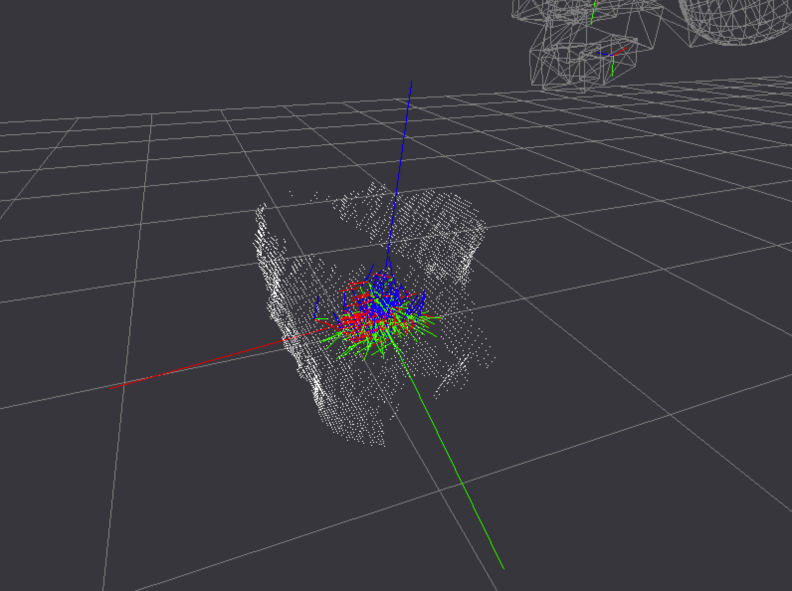
\includegraphics[height=5.0cm,width=.48\columnwidth]{../media/iros/2013/img/from_rss/high_dim_filter}
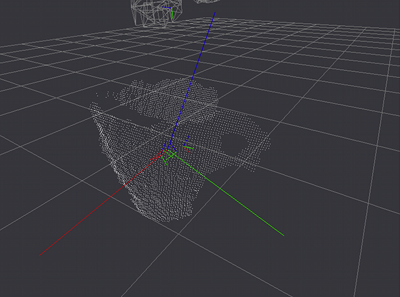
\includegraphics[height=5.0cm,width=.48\columnwidth]{../media/iros/2013/img/from_rss/low_dim_filter}
}
\vspace{0.8mm}
\centerline{
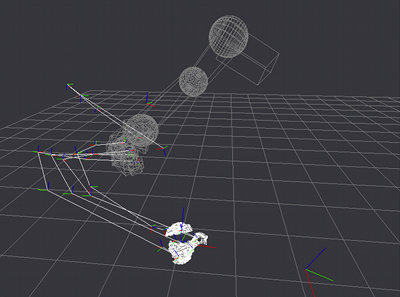
\includegraphics[height=5.0cm,width=.48\columnwidth]{../media/iros/2013/img/from_rss/unoptimised_trajectory}
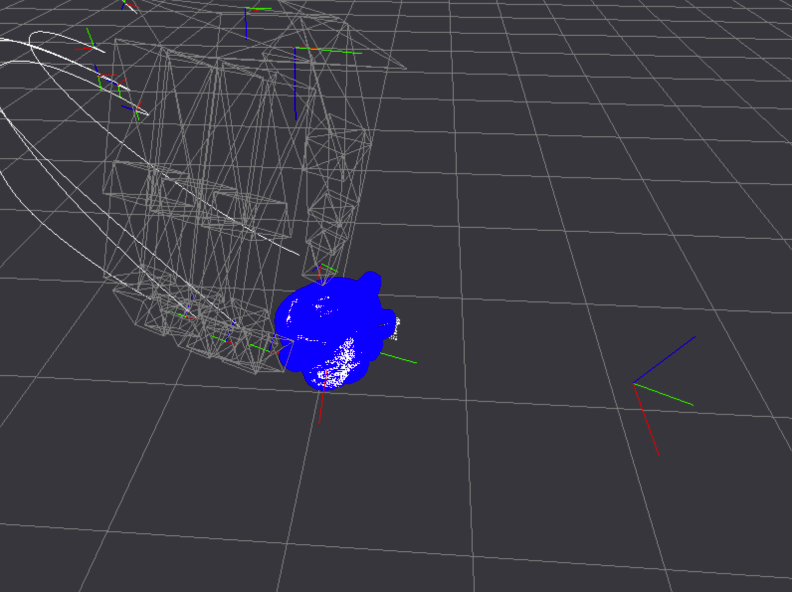
\includegraphics[height=5.0cm,width=.48\columnwidth]{../media/iros/2013/img/from_rss/optimised_trajectory}
}
\caption[IG planner for dexterous grasping]{Top row: The high dimensional belief state used to track object pose (left); the low dimensional filter used for planning (right). Bottom row: The unoptimised PRM plan for fingers and wrist (left); the optimised and smoothed trajectory (right).}
\label{fig:spam.plan.example}
\end{figure}

\subsection{Planning a trajectory to maximise information gain}\label{sec:ch06:heuristic}

The implementation of this planner uses a modified version of Probabilistic Roadmap (PRM),~\citep{bib:kavraki_1996}, to plan trajectories and detect collisions. As discussed in Sec.~\ref{subsec:ch03:multi_query}, the PRM algorithm is composed of two phases: i) \emph{learning phase}, in which a connected graph $\mathbf{G}$ of obstacle-free configurations of the robot is generated and, ii) \emph{query phase}, in which a path is searched for a given pair of configurations $x_{root},x_{goal}$. However the computational cost for the learning phase grows very fast with respect to the dimensionality of the problem. This planner therefore incrementally builds connections between neighbouring nodes during the query phase. 
Given a pair $\langle x_{root}, goal\rangle$ which describes the root state in configuration space, $\mathbb{R}^n$, and goal state in workspace, $SE(3)$, of the trajectory, this planner uses an A* algorithm to find a minimum cost trajectory in obstacle-free joint space according to:
\begin{equation}
c(x) = c_1(x,x_{root}) + c_2(x,x',\hat{x}_{goal})
\end{equation} 
where $x,x'\in\mathbb{R}^n$ and $x'\in Neighbour(x)$, $\hat{x}_{goal}$ is a reachable goal configuration for the robot computed by inverse kinematics, $c_1(x,x_{root})$ is the cost-to-reach $x$ from $x_{root}$ and $c_2(x,x',\hat{x}_{goal})$ is a linear combination of the cost-to-go from $x$ to a neighbour node $x'$ and the expected cost-to-go from $x'$ to the target. I implemented $c_1(\cdot)$ as a cumulative discounted and rewarded travelled distances. More specifically, I define 
%Initially a random graph, $\mathbf{G}$, of robot configurations in obstacle-free space is generated and then a path to a given goal state is searched according to some user defined heuristic. 
%Given a pair $\langle x_{root}, goal\rangle$ which describe the root state in configuration space, $\mathbb{R}^n$, and goal state in workspace, $SE(3)$, of the trajectory, our PRM-based algorithm finds a joint space trajectory as follows:
%\begin{itemize}
%\item adds $x_{root}$ to $\mathbf{G}$
%\item finds a obstacle-free configuration $\hat{x}_{goal}$ which is a reachable goal configuration for the robot
%\item evaluates each node $x$ in the graph $\mathbf{G}$ according to 
%\begin{equation}
%\begin{aligned}
%c_1(x,x_{root},\hat{x}_{goal})=&\alpha d(x,x_{root})\\
%&+\beta d(x,\hat{x}_{goal})+\gamma d_{cfg}(x)
%\end{aligned}
%\end{equation} 
%\item starting from $x_{root}$ finds all its neighbouring nodes within a given threshold and compute the follows cost-to-go function
\begin{equation}\label{eq:cost2}
\begin{aligned}
c_2(x,x',\hat{x}_{goal})=\alpha d_{bound}(x,x') +\beta &d(x',\hat{x}_{goal})\\
&+\gamma d_{cfg}(x)
\end{aligned}
\end{equation} 
%\item finds a path from $x_{root}$ to $\hat{x}_{goal}$ which minimises $c_2(\cdot)$ using A* algorithm
%\end{itemize}
where $\alpha,\beta,\gamma\in\mathbb{R}$, $d(\cdot)$ is a distance function in $SE(3)$ which linearly combine rotational and translational distances in workspace\footnote{For the sake of simplicity, I reduce the mathematical notation by writing $d(x,x')$ instead of d(W(x),W(x')).}. For $d_{bound}(\cdot)$, let $\mathcal{B}_n(r)=\{x\in\mathbb{R}^n|x^Tx\leq r^2\}$ and $\mathcal{B}(r_{l},r_{a})=\{A=[\begin{smallmatrix}R&p\\ 0&1\end{smallmatrix}]\in SE(3)|p^Tp\leq r_{l}^2\text{ and } 1-\langle Q(R),Q(R)\rangle\leq r_{a}^2\}$\footnote{I simplified the notation $\mathcal{B}_{SE(3)}(\cdot)$ in $\mathcal{B}(\cdot)$ for pratical reasons.} denote repectively the $r$-ball in $\mathbb{R}^n$ and in $SE(3)$, then $b_{bound}(x,x')$ is defined as %$\zeta d(x,x')+(1-\zeta)||x-x'||_2$ with $\zeta\in(0,1)$ if $\mathcal{W}(x)-W(x')\in\mathcal{B}_{SE(3)}(r)$ and $x-x'\in\mathcal{B}_n(r')$ or $+\infty$ otherwise.
$$
d_{bound}(x,x')=
\begin{cases}
\psi(x,x')& \text{if }W(x)-W(x')\in\mathcal{B}(r_{l},r_{a}) \\
& \text{and }x-x'\in\mathcal{B}_n(r) \\
+\infty & \text{otherwise}
\end{cases}
$$
where $Q(\cdot)$ is the Quaternion operator for $R\in SO(3)$, $\langle q_1,q_2\rangle$ is the inner product of two quaternions, $r_{l}, r\in\mathbb{R}, r_{a}\in (0,1)$, and $\psi(x,x')=\zeta d(x,x')+(1-\zeta)||x-x'||_2$ with $\zeta\in(0,1)$.
%is an \emph{ad-hoc} distance function that takes into account also distance in the joint space and has the good property of penalising pairs of configurations far away from each others 
Finally, $d_{cfg}(\cdot)$ is a function which penalises dangerous configurations of the robot (i.e. close to joint limits). %Our PRM-based algorithm uses $d_{bound}(\cdot)$ and $d_{cfg}(\cdot)$ to generate edges only between safe robot's configurations (PRM nodes) which are close enough in joint space, and transitions between one configuration and the other can be easily computed by inverse kinematic.

I redefine the heuristic $c_2(\cdot)$ in order to reward informative tactile explorations while attempting to reach the goal state (described as a target configuration of the manipulator). 
%Let $x\in G$ define a obstacle-free configuration of the robot in the PRM, then iteratively the PRM algorithm minimises the following cost function:
% \begin{equation}\label{eq:modifiedcost2}
%\min_{x'\in G}{\alpha \mathcal{J}(x, x', p^{1:k})d_{bound}(x,x')+\beta d_Q(x',\hat{x}_{goal})+\gamma d_{cfg}(x')}
%\end{equation}
%
%Our main contribution is the definition of a new set of heuristics which encode the uncertainty over the object pose. We define,  
%\begin{equation}\label{eq:newcost1}
%\begin{aligned}
%\bar{c}_1(x,x_{root},\hat{x}_{goal},Q)=&\alpha d(x,x_{root})\\
%&+\beta d_Q(x,\hat{x}_{goal})+\gamma d_{cfg}(x)
%\end{aligned}
%\end{equation}
%and 
\begin{equation}\label{eq:newcost2}
\begin{aligned}
\bar{c}_2(x,x',\hat{x}_{goal},A,p^{1:k})=&\alpha \mathcal{J}(x,x',p^{1:k})d_{bound}(x,x')\\
&+\beta d_A(x',\hat{x}_{goal})+\gamma d_{cfg}(x')
\end{aligned}
\end{equation}
where $A$ is the diagonal covariance matrix of the sampled states, for any column vector $a,\mu\in\mathbb{R}^n$, $d_A(a, \mu)=\sqrt{(a-\mu)^TA^{-1}(a-\mu)}$ is the Mahalanobis distance centered in $\mu$ and $\mathcal{J}(x,x',p^{1:k})\in(0,1]$ is a factor which rewards trajectories with a large difference between expected observations if the object is at the expected location, $p^1$, versus observations that would be expected if the object is at other poses, $p^{2:k}$, sampled from the distribution of poses associated with the object's positional uncertainty:
\begin{equation}\label{eq:modifiedcost}
\mathcal{J}(x,x',p^{1:k})=\frac{1}{k-1}\sum_{i=2}^k{e^{-\Phi(x,x',p^i)}}
\end{equation}
where:
$$
\Phi(x,x',p^i)=||h_t(x,x',p^i)-h_t(x,x',p^1)||_2
$$
for each $i\in[2,k]$ and $h_t(x,x',p^i)$ is sequence of probability of reading a contact travelling from state $x$ to $x'$. In this implementation $h_t(x,x',p^i)=h(x',p^i)$. In other words, I evaluate the likelihood of making a contact while moving from state $x$ to $x'$ as the likelihood of making a contact only in the next state $x'$.
Note that this observational model is designed to conserve (\ref{eq:newcost2}) as in (\ref{eq:cost2}) when the likelihood of observing a tactile contact is zero. In fact, for robot configurations in which the distance to the sampled poses is larger than a threshold, $d_{max}$, the cost function $\mathcal{J}(\cdot)$  is equal to 1. However I also encode uncertainty in the second factor of the heuristics, $d_A(\cdot)$, which evaluates the expected distance to the goal configuration. In this way the planner also copes with pose uncertainty at the early stages of the trajectory, when the robot is still too far away from the object to observe any contacts. 

\subsection{Planning for Dexterous manipulator}

In order to compute a dexterous trajectory which allows us to plan movement for both arm and fingers we need to break down the curse of dimensionality or, equivalently, increase the number of sampled configurations to properly cover the configuration space. 

The proposed solution is to build a hierarchical planner. First a PRM is constructed only in the arm configuration space in order to find a global path between the $x_{root},\hat{x}_{goal}$. It is worth noticing that in this phase the rest of the joints of the manipulator are interpolated in order to have a smooth passage from $x_{root}$ to $\hat{x}_{goal}$. Then the planned trajectory is refined by constructing a new PRM in the entire configuration space of the manipulator (e.g. arm + hand joint space) along the global path. In other words, this approach limits the new PRM to explore only the subspace nearby the configurations which compose the global path.  
Subsequently an optimisation procedure is executed along the trajectory to generate a smoother transition from one configuration to the next.

This approach enable us to plan dexterous reach-to-grasp trajectories up to 21 DoF with only 1,000 sampled configurations. Note that this is the same order of magnitude that it is used in practise for planning trajectories of much simpler 6 DoF robot manipulators. 

\subsection{Belief update}

Once a trajectory is executed and a real (unexpected) observation $y$ is detected, the belief state is updated according to the Bayes' rule. The belief state is represented as a set of $N$ particles $b_t=\{b_t^z\}_{z=1}^{N}$. In a particle filter fashion the weight of each particle $b_t^z$, $z\in\{1,\ldots,N\}$ is updated as follows
$$
Pr(y|x, b_t^z)=\prod_{j\in\hat{M}}{Pr(y_{t}(j)|x_{t}(j),b_t^z)}
$$
and then re-sampling is performed to generate a posterior distribution $b_{t+1}$ as new set of particles $\{b_{t+1}^z\}_{z=1}^{N}$.

In simulation this approach assumes that there are no false detections. However it is possible to distinguish whether or not a contact occurs between the object to be grasped and the robot's end-effector. For example, in case a contact with the environment is detected, the algorithm skips the belief update step and moves the robot back to a safe configuration before triggering the re-planning.


%---------------------------------------------------------------------------------------------------------------------
% 	EXPERIMENTS
%---------------------------------------------------------------------------------------------------------------------
%---------------------------------------------------------------------------------------------------------------------

\section{Results}\label{sec:ch06:results}

\begin{figure*}[t!]
  \centering
  \begin{subfigure}[t]{0.4\textwidth}
       \includegraphics[height=3.9cm,width=5.4cm]{../media/iros/2013/img/replanning/1}
       \caption{}\label{fig:replan_1}
  \end{subfigure} 
  \quad
  \begin{subfigure}[t]{0.4\textwidth}
     \includegraphics[height=3.9cm,width=5.4cm]{../media/iros/2013/img/replanning/3}
     \caption{}\label{fig:replan_3}
  \end{subfigure}
  \vspace{2mm}
  \begin{subfigure}[t]{0.4\textwidth}
       \includegraphics[height=3.9cm,width=5.4cm]{../media/iros/2013/img/replanning/2}
       \caption{}\label{fig:replan_2}
  \end{subfigure} 
  \quad
  \begin{subfigure}[t]{0.4\textwidth}
     \includegraphics[height=3.9cm,width=5.4cm]{../media/iros/2013/img/replanning/6}
     \caption{}\label{fig:replan_6}
  \end{subfigure}
  \vspace{2mm}
  \begin{subfigure}[t]{0.4\textwidth}
       \includegraphics[height=3.9cm,width=5.4cm]{../media/iros/2013/img/replanning/5}
       \caption{}\label{fig:replan_5}
  \end{subfigure} 
  \quad
  \begin{subfigure}[t]{0.4\textwidth}
     \includegraphics[height=3.9cm,width=5.4cm]{../media/iros/2013/img/replanning/8}
     \caption{}\label{fig:replan_8}
   \end{subfigure}
   \vspace{2mm}  
   \begin{subfigure}[t]{0.4\textwidth}
       \includegraphics[height=3.9cm,width=5.4cm]{../media/iros/2013/img/replanning/7}
       \caption{}\label{fig:replan_7}
  \end{subfigure} 
  \quad
  \begin{subfigure}[t]{0.4\textwidth}
     \includegraphics[height=3.9cm,width=5.4cm]{../media/iros/2013/img/replanning/9}
     \caption{}\label{fig:replan_9}
  \end{subfigure}
%\centerline{
%\includegraphics[height=5.0cm,width=.48\columnwidth]{../media/iros/2013/img/replanning/1}
%\includegraphics[height=5.0cm,width=.48\columnwidth]{../media/iros/2013/img/replanning/3}
%}
%\vspace{.8}
%\centerline{
%\includegraphics[height=5.0cm,width=.48\columnwidth]{../media/iros/2013/img/replanning/2}
%\includegraphics[height=5.0cm,width=.48\columnwidth]{../media/iros/2013/img/replanning/6}
%}
%\vspace{.8}
%\centerline{
%\includegraphics[height=5.0cm,width=.48\columnwidth]{../media/iros/2013/img/replanning/5}
%\includegraphics[height=5.0cm,width=.48\columnwidth]{../media/iros/2013/img/replanning/8}
%}
%\vspace{.8}
%\centerline{
%\includegraphics[height=5.0cm,width=.48\columnwidth]{../media/iros/2013/img/replanning/7}
%\includegraphics[height=5.0cm,width=.48\columnwidth]{../media/iros/2013/img/replanning/9}
%}
\caption[SPAM-PLAN execution]{The belief states shown are the low dimensional belief states sub-sampled from the corresponding high dimensional belief states. Top row: Initial belief state~\subref{fig:replan_1}, first contact~\subref{fig:replan_3}. Second row: updated belief state from first contact~\subref{fig:replan_2}, second contact~\subref{fig:replan_6}. Third row: updated belief after second contact~\subref{fig:replan_5}, third contact~\subref{fig:replan_8}. Bottom row: updated belief after third contact~\subref{fig:replan_7}, executed reach-to-grasp pose~\subref{fig:replan_9}.}
\label{fig:spam.exec.example}
\end{figure*}

\begin{table*}[t!]
\centering
\caption{Experimental results in simulation}
\begin{tabular}{ | c | c || c || c | c || c | c |}
\hline
\hline
\multicolumn{2}{ |c|| }{Initial error} & 	Single & \multicolumn{2}{ c|| }{ReGrasp} & \multicolumn{2}{ c| }{ReGrasp+IG} \\\hline
Lin (m) & Ang (quat) &  &	Iterations	&	FCA	&	Iterations	& FCA \\ \hline
0.055909		& 	0.006344	& 	success	&	1	&	0.006301	&	2	&	0.005876 \\ \hline
0.05343		&	0.012268	&	success	&	1	&	0.006072	&	2	&	0.00649 \\ \hline
0.057804		&	0.013443	&	success	&	1	&	0.005996	&	2	&	0.005308 \\ \hline
0.060809		&	0.016942	&	failure	&	2	&	0.000452	&	1	&	0.000911 \\ \hline
0.058412		&	0.017696	&	success	&	1	&	0.008286	&	1	&	0.006266 \\ \hline
0.05996		&	0.019115	&	failure	&	4	&	0.005679	&	1	&	0.008111 \\ \hline
0.05755		&	0.019915	&	success	&	1	&	0.005936	&	1	&	0.003597 \\ \hline
0.05815		&	0.020103	&	failure	&	7	&	0.003868	&	1	&	0.003737 \\ \hline
0.059598		&	0.021463	&	failure	&	3	&	0.007579	&	1	&	0.006105 \\ \hline
0.061404		&	0.023431	&	success	&	1	&	0.007397	&	1	&	0.006409 \\ \hline
0.063758		&	0.025339	&	success	&	1	&	0.007959	&	2	&	0.002738 \\ \hline
0.059935		&	0.054883	&	failure	&	2	&	0.005933	&	2	&	0.00752 \\ \hline
\hline
\end{tabular}
\label{tab:ch06_results}
\end{table*}


In this work I aim to show that sequential re-planning is capable of achieving higher successful grasp rates than single grasp attempts, in presence of non-Gaussian object-pose uncertainty in 6 dimensions. I also show that planning trajectories that maximise information gain requires fewer re-planning iterations to achieve a grasp with the same order of magnitude of grasp quality.  

The algorithm has been tested by running 12 trials in a virtual environment. Each trial has a different initial probability density over the object pose, so to test the ability of different strategies to achieve a grasp configuration in which it is possible to obtain force closure grasp despite the pose uncertainty. In these experiments, after an unexpected observation occurs, the robot is always moved back to the initial configuration shown in Fig.~\ref{fig:justin} (left image).

Table~\ref{tab:ch06_results} summarises the data collected in the experiments. First the algorithm computed the error in the initial estimation of the object pose with respect to the ground truth, which is available in the simulation environment. This error is decomposed into translational and rotational components. The translational component measures  displacement as Euclidian distance in a 3 dimensional space between the estimated location and the ground truth. The rotational or angular displacement is evaluated using the quaternion representation.

Next, three different algorithms are performed: i) an open-loop trajectory towards the expected object pose without re-planning, ii) a sequential re-planning algorithm, which exploits contact observations gathered during the previous grasp attempt, but does not plan trajectories specifically to maximise information gain (ReGrasp) and iii) sequential re-planning with reach-to-grasp trajectories which are specifically optimised to maximise the expected tactile information gain, while also achieving the desired grasp configuration (ReGrasp+IG). Column 3 in table~\ref{tab:ch06_results} shows the rate of successful attempts for the open-loop trajectory. Columns 4 and 5 show that successive re-planning enables us to achieve a grasp in cases when the open-loop strategy fails. The table presents both the number of (re-)planning iterations and the grasp quality value once a force closure grasp is achieved. Finally, columns 6 and 7 show that, planning trajectories which maximise information gain, reduces the number of re-planning iterations required to achieve a successful grasp while producing the same order of magnitude of grasp quality. 
Note that, for all the trials, the nominal grasp quality computed on the object in the nominal pose is 0.006920. 

An interesting case is shown in the 8th row of Table~\ref{tab:ch06_results}. In this trial a single attempt fails while ReGrasp requires 7 iterations to generate a quite poor force closure. Instead using ReGrasp+IG produces a successful trajectory at the very first attempt, although the grasp quality does not improve in this specific case.

To illustrate the behaviour of the re-planning system, Fig.~\ref{fig:spam.exec.example} shows a typical sequence generated by one simulation trial. The algorithm assumes a known point cloud model of the object shape, and uncertainty in the object pose. In this trial the robot observes the object as a point cloud and applies a model fitting process described in~\citep{bib:uli_cviu_2011}. The model fitting process is stochastic and so the resulting pose of the object is uncertain. Multiple poses are sampled by repeating this process, and to obtain a belief state consisting of the resulting set of possible poses of the object. A trajectory is then planned to achieve a given grasp on the object. At each step a trajectory for the wrist and fingers are generated that will move to the desired grasp, while deviating from a minimum length trajectory to maximise information gathered through tactile observations. The belief state is updated and re-planning occurs each time a tactile contact is made. In this example three separate contacts are made during reach-to-grasp trajectories. In each instance the trajectory is re-planned given the new belief state. After three contacts the fourth trajectory achieves a configuration suitable for grasping.

A drawback of ReGrasp+IG is the computational time. In the experiments ReGrasp requires on average $\sim7$ seconds to plan a trajectory as compared to $\sim200$ seconds for ReGrasp+IG. ReGrasp+IG adds extra computation during the query phase of the PRM algorithm in order to compute the likelihood of reading a contact, which requires finding the closest surface to the finger tips for each hypothesis (represented as point clouds) every time a node in the PRM is in a neighbourhood of the uncertain region. In the next chapter, I will present a fast and efficient KD-tree based algorithm for collision detection for non-convex objects represented as point clouds (Sec.~\ref{sec:ch07:non_convex_obj}) to overcome this extra computation in the planning phase.

%---------------------------------------------------------------------------------------------------------------------
% 	CONCLUSION AND FUTURE WORK
%---------------------------------------------------------------------------------------------------------------------
%---------------------------------------------------------------------------------------------------------------------

\section{Conclusion} 
\label{sec:ch06:summary}

In this chapter I have shown how to solve the problem of dexterous grasping of objects with uncertain pose by using information gain re-planning.

I have proposed a method for tactile information gain planning for dexterous, high DoF manipulators by using i) a hierarchical PRM planner which encodes informational measure in its segments, and ii)  a method for sequentially refining pose uncertainty, by using tactile observations gathered
during unsuccessful grasp attempts. This approach enables planning for robot manipulators with 21 DoF and non-Gaussian object pose uncertainty in 6 dimensions.

I have also shown how sequential re-planning
can achieve better quality grasps than single attempts to directly grasp an
object at its expected pose, and that re-planning with trajectories
designed to maximise tactile information gain, achieves successful grasps
with fewer iterations than sequential attempts to grasp directly towards
the object's (sequentially updated) expected pose.

%i) a method for sequentially updating non-Gaussian
%beliefs in 6 dimensions about the pose of an object, by using tactile observations gathered
%during unsuccessful grasp attempts, ii) how sequential re-planning
%can achieve better quality grasps than single attempts to directly grasp an
%object at its expected pose, and iii) that re-planning with trajectories
%designed to maximise tactile information gain, achieves successful grasps
%with fewer iterations than sequential attempts to grasp directly towards
%the object's (sequentially updated) expected pose. In addition we have also proposed a hierarchical PRM algorithm to enable planning of dexterous reach-to-grasp trajectory for manipulators with high DoF.

This work extends that of \citep{bib:platt_csail_2011}, 
%which offers a way to avoid the complexity of planning in a high dimensional belief space
which offers a way to avoid the complexity of planning in a high dimensional belief space. It does
this in two ways, i) by approximating the informational value of
actions from a low-dimensional subspace of the belief state; and
ii) by embedding that informational value into the physical
space. This enables standard motion planning techniques to trade off
directly between information gain and achievement of the goal pose for
the manipulator.

%\subsection{Future Work}
%
%We aim to extend our observational model in order to cope with non-static objects by using a physics simulator as a forward model which enable us to predict how the object behaves under a hand-object interaction. In addition, we are interested in extending sensing abilities of the robot by using tactile sensors on the robotic hand.
%We also aim to investigate our re-planning approach with different withdrawing policies, instead of moving the robot back to its starting configuration at each iteration, e.g. adjusting fingers and wrist configurations to gain even more contact information.

%In this chapter we have shown how our previous work on planning
%information gathering trajectories for a 7 dof manipulator can be
%extended. Our contributions relative to our previous work are: i) to
%extend the planning process in an incremental fashion to plan first
%the TCP trajectory, and then the finger trajectories; ii) to include
%both the belief updating in 6 dimentions and replanning steps; iii) to present an
%initial result from simulation. In this work we have extended previous
%work on planning under uncertainty for grasping to Dexterous grasping
%with a high degree of freedom hand.  
%The principle of the approach,
%adapted from \citep{bib:platt_csail_2011} avoids planning in a high
%dimensional belief space with the intractability that entails. It does
%this in two ways, first by approximating the informational value of
%actions from a low-dimensional subspace of the belief state; and
%second by embedding that informational value into the physical
%space. This enables standard motion planning techniques to trade off
%directly between information gain and achievement of the goal pose for
%the manipulator. Our future work will be to evaluate the performance
%of this approach in both simulated and real environments.

%\section*{ACKNOWLEDGMENT}
%
%\noindent We gratefully acknowledge the support of the EC FP7 ICT programme
%through the FP7 projects GeRT (248273) and PaCMan (600918).































